\chapter{The overview}
\label{sec:overview}

\textbf{Summary and discussion of all results.}

In the discission above we have covered in great detail the possibilites of high-entropy silicides based on the $\beta-$ \ch{FeSi2} unit cell with twice as many silicon atoms to 3d elements. The primary outcome and conclsion of this research was that particularly the combination of Cr, Fe, Mn and Ni resulted in superiour properties in the light of the motivatian behind this project. The next question we wish to answer is if ihe promising results of the CFMN system be reproduced in other symetries. In this section we will implement the CFMN composistion in crystal structures based on hexagonal \ch{CrSi2} ($P6_{42\Bar{2}}$), both tetragonal and orthorombic \ch{Mn16Si28} ($P\Bar{4}c2 and$, $Pcca$), and trigonal \ch{Fe2Si} ($P\Bar{3}m1$) where we test the CFMN system to varying metal and silicon ratioes, and crystal structures. As before, the total energy, enthalpy of formation and magnetic moment per atom can be found bellow in table ..
\begin{table}[h!]
\begin{tabular}{@{}cccccc@{}}
\toprule
            & \multicolumn{2}{c}{Total energy per energy} & Enthalpy of formation & \multicolumn{2}{c}{Mag per atom} \\ \midrule
CrSi2       & -6.4837               & 0.0087              & -8.1205             & 0.0887          & 0.0387         \\
MnSi        & -6.6658               & 0.0071              & -9.1848             & 0.0687          & 0.0398         \\
Fe2Si       & -7.5082               & 0.0107              & -10.2474            & 0.3848          & 0.0588         \\ \bottomrule
\end{tabular}
\end{table}

\textbf{CrSi2}
From our calculations with PBE DFT we find the bulk crsi2 material to be an indirect semiconductor with a band gap of 0.33 eV, slightly bellow the listed value of 0.36 eV in materials project \textbf{cite}, suprinsingly we find a smaller gap of 0.32 eV from the SCAN functional. The compound is also nonmagnetic in agreement with materials project. Fore the bulk material we employed a 9 atom cell, with 6 silicon and 3 cr atoms, from this we generated SQSs of 72 atoms with the same ratio.  \textbf{Include toten per atom for the unit cell? and figure of SQS + unit cell?}. For this given composistion and system we observe very similar results to that of the composistions discussed above, the eigenvalues of several SQSs report a small band gap, but its not apperant from neither the density of states or from the bandgap.py script of pymatgen. Additiontly, we can not repreoduce the gap with the SCAN functional, as was possible for the CFMN (fesi2) system.   

\textbf{MnSi}
In the tetragonal configuration, the bulk material is a nonmagnetic indirect semiconductor with a band gap of 0.76 eV acoording to our PBE calculations,  and 0.78 eV from SCAN. Materials project find a band gap of 0.76 eV, in good agreement with our own PBE results. The unit cell consist of 44 total atoms, 16 manganese and 28 silicon. In the orthoromibic cell, with equal number of elements we find a band gap of 0.76 eV (0.77 ev SCAN) as well. In contrast, the CFMN alloy of both these cells produce metalic compounds. It should be noted that structures B and D in the tetragonal ssystem did not fully relax, same for D in the orthorombic cell, so these results could be inaccurate.   

\textbf{Fe2Si}
In this cell, we drasticly alter the metal-silicon ratio, this is seen both in the band gap and magnetic properties of the material. The magnetic moment of this cell consisting of 4 iron atoms and 2 silicon atoms is 0.67, from the iron atoms. This magnetic charachter can also be observed from the discrepency between the two spin channels. In spin down we find a band gap of 0.21 eV, while there is no gap in spin up. This gap can also be seen in the density of states \textbf{Include figure}. This however is an abnormal result in regard to other experimental work and littereature on the Fe2Si \textbf{cite $https://www.sciencedirect.com/science/article/pii/S0925838816329796?casa_token=g9DRpU9IClcAAAAA:6Gd12A4Kh9J2igUWMVwHN8OSIKzD27VACA052FNsSAWhRY6PELWdVEPbiF8OtQ3eJEAbvQ8X0g$}. Our results are subject to errors, particularly we note that the eigenvalues used to calculate the gap contain nonphysical values in the spin down channel. However, the gap is evident in the density of states thus we include the result in this report, but acknowlendge the uncertainties revolving the value. 

From this unit cell we generate 54 atom SQSs. From table .. we see that the magnetic nature remains, producing the overall highest magnetic moment of all studied supercells, which is not a surprising result considering the 3d metal to silicon ratio. \textbf{More on magnetic and total energy.} The magnetism can also be seen in the difference between the two spin channels, the bands where the occupancy transistion from 1 to 0, ie occupied to not occupied is very different. In the most magnetic supercell D, we saw a distance of 22 bands between the spin down transistion and spin down transistion. Most supercells are metals from our PBE calculations. B and D show a very small gap of around 0.01 eV in one spin channel.  In E we find a very narrow gap semiconductor with a total gap of 0.002 eV. This gap is surrounded by the same uncertainties as discussed previosly.  

\begin{figure}[H]
\centering
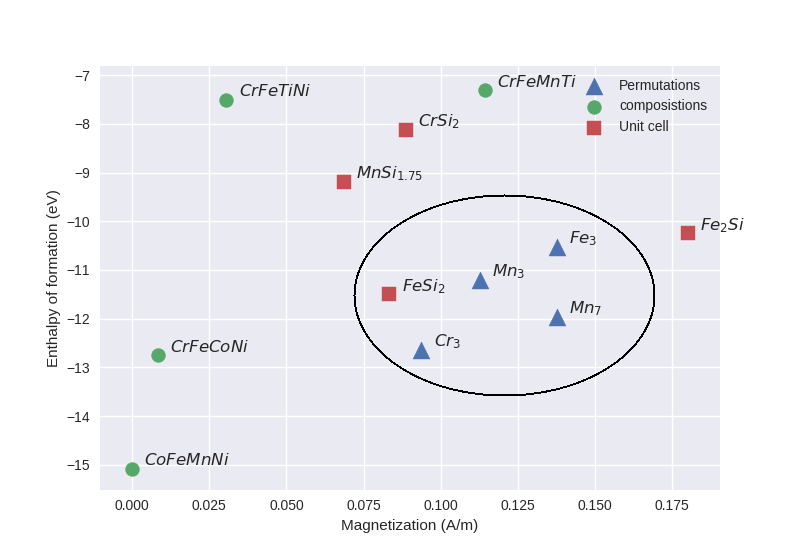
\includegraphics[width=\textwidth]{results/diagram.png}
\end{figure}